\chapter{Contactos metal-semiconductor}

Los materiales estudiados hasta el momento se encuentran en estado de equilibrio térmico (sin tensión aplicada, temperatura constante, sin luz). Los diagramas de bandas en equilibrio para el silicio intrínseco, silicio tipo n y silicio tipo p se muestran en la Figura \ref{detalle_bandas_equilibrio}.

\begin{figure}[H]
    \centering
    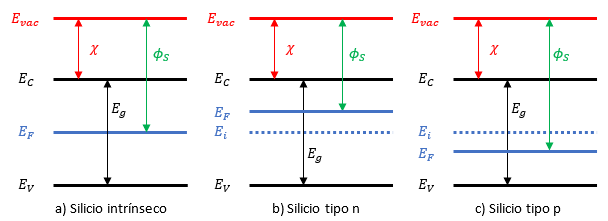
\includegraphics{figuras/bandas_en_equilibrio_detalle.png}
    \caption{Diagramas de banda del silicio en equilibrio térmico, sin tensión aplicada.}
    \label{detalle_bandas_equilibrio}
\end{figure}

Las bandas son planas indicando que la energía es la misma en cualquier posición del cristal y que la energía $E$ no varía con la posición $x$. En los diagramas, la energía está definida para un electrón, el eje vertical indica que la energía aumenta y que el potencial disminuye.

Cuando el material se encuentra en condiciones fuera de equilibrio, por ejemplo, al unir dos materiales distintos, las bandas se curvan y se produce una transferencia de energía. En este capítulo se estudian los dos tipos principales de contacto metal-semiconductor: el \textbf{contacto Schottky} o contacto rectificante, y el \textbf{contacto óhmico} o no rectificante.


\newpage
\section{Deformación de bandas}

Cuando se asumen condiciones fuera de equilibrio térmico, por ejemplo, cuando se aplica energía externa en forma de temperatura, luz, tensión aplicada, o cualquier otra fuente de energía externa que altera la electrostática del material, existe \textbf{deformación de bandas}. Esto sucede en los siguientes dos escenarios:

\subsection{Tensión aplicada en una sección del material}

La tensión eléctrica es una diferencia de potencial. El potencial eléctrico V es una forma indirecta de describir la energía potencial E, y se cumple que:

\[ E = -q V \]

Un potencial positivo desplaza las bandas hacia abajo. Un potencial negativo desplaza las bandas hacia arriba. Si hay una diferencia de potencial entre dos puntos, las bandas se doblan por continuidad.

\subsection{Contacto de dos materiales con distintos niveles de energía}

\begin{itemize}
    \item \textbf{Contacto de dos metales distintos (efecto Seebeck):} cada metal tiene una función de trabajo $\phi_M$ distinta, y al unir ambos materiales, se crea una diferencia de potencial. Este efecto es utilizado para fabricar sensores de temperatura, conocidos como termopares o termocuplas.
    \item \textbf{Contacto metal-semiconductor (contacto óhmico y contacto Schottky):} al unir un metal con un semiconductor, se crean dos tipos de contactos: el contacto óhmico es resistivo y permite el paso de corriente en ambas direcciones, el contacto Schottky o rectificante permite el paso de corriente en una sola dirección, bloqueando la corriente en sentido contrario.
    \item \textbf{Contacto semiconductor-semiconductor (unión PN o diodo):} al unir dos bloques de silicio, uno de tipo p y el otro de tipo n, se obtiene un contacto rectificante.
\end{itemize}


\newpage
\section{Electrostática}

Cuando hay un campo eléctrico $\mathcal{E}$ en el semiconductor, el diagrama de bandas se deforma. Los niveles de energía dependen ahora de la posición $x$.

\subsection{Tensión}

Un potencial positivo desplaza las bandas hacia abajo:

\[ E = -qV \]

El potencial se calcula con respecto a un nivel de referencia:

\[ V = -\dfrac{1}{q} (E_c - E_{ref}) \]

El nivel de referencia es un nivel de energía arbitrario, debido a que un potencial siempre se mide con respecto a un potencial de referencia que también es arbitrario. Por ejemplo, en un circuito con dos resistencias en serie, si se quiere medir la tensión en algún punto, la terminal de referencia del voltímetro se puede conectar a tierra o a cualquier otro punto del circuito.

\textbf{Por lo tanto, el potencial $V$ es un espejo de la banda de conducción $E_c$.}


\subsection{Campo eléctrico}

El campo eléctrico $\mathcal{E}$ se define como:

\[ \mathcal{E} = -\nabla V = \dfrac{-dV}{dx} \]

De modo que es válido escribir

\[ \mathcal{E} =  \dfrac{1}{q} \dfrac{dE_c}{dx} = \dfrac{1}{q} \dfrac{dE_v}{dx} = \dfrac{1}{q} \dfrac{dE_i}{dx} \]

\textbf{Por lo tanto, el campo eléctrico $\mathcal{E}$ es la primera derivada de la banda de conducción $E_c$.}


\subsection{Carga}

La carga eléctrica se relaciona con el campo eléctrico por medio de la \textbf{Ecuación de Poisson}:

\[ \dfrac{d\mathcal{E}}{dx} = \dfrac{\rho}{\epsilon_0 \epsilon_r} = \dfrac{q N_D}{\epsilon_0 \epsilon_r} \]

Donde:

$\epsilon_0$: permitividad del vacío ($8.85 \times 10^{-14}\ F\cdot{}cm^{-1}$)

$\epsilon_r$: permitividad relativa (Si: 11.7, Ge: 16.2)

$\rho$: densidad de carga eléctrica [$C/cm^{-3}$]

\textbf{Por lo tanto $\rho$ es la primera derivada del campo eléctrico, y es la segunda derivada de la banda de conducción $E_C$.}

En el diagrama de bandas de la Figura \ref{bandas-doblamiento-vext} existe una diferencia de potencial entre el extremo $x=0$ y el extremo $x=l$, y por lo tanto las bandas tienen distinto nivel de energía. En el diagrama se observan las relaciones entre todas las variables.

\begin{figure}[H]
    \centering
    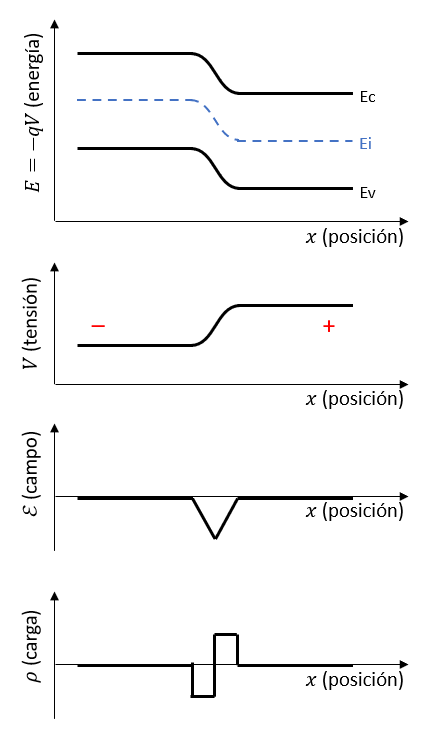
\includegraphics{figuras/bandas-doblamiento-vext.png}
    \caption{Gráficas para la energía $E$, el potencial $V$, campo eléctrico $\mathcal{E}$, y carga $\rho$.}
    \label{bandas-doblamiento-vext}
\end{figure}

\section{Doblamiento de bandas en contactos}

Al unir dos materiales distintos, existe un \textbf{intercambio de portadores} que alinea los niveles de Fermi de ambos materiales. La función de trabajo en ambos materiales permanece constante. \textbf{En estado de equilibrio, después del movimiento de cargas, el nivel de Fermi es constante y totalmente horizontal.}

En la Figura \ref{tipos_de_contactos} se muestran ejemplos de dos tipos de contactos, el primero entre silicio p y silicio n, el segundo entre un metal y silicio tipo n.

\begin{figure}[H]
    \centering
    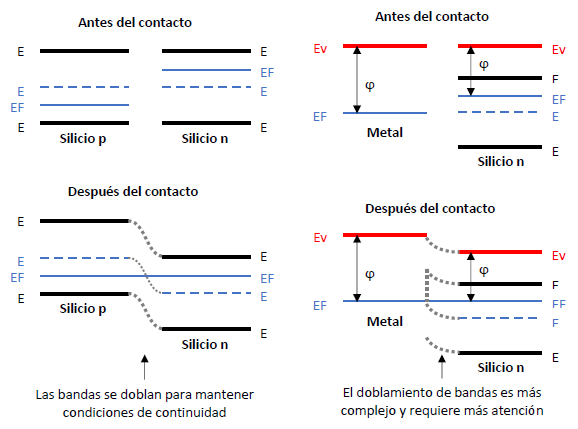
\includegraphics{figuras/tipos_contactos_MS_SS.png}
    \caption{Ejemplos de la deformación de bandas en un contacto semiconductor-semiconductor y en un contacto metal-semiconductor.}
    \label{tipos_de_contactos}
\end{figure}


\newpage
\section{Contactos metal-semiconductor}

Si se une un metal con un semiconductor, se puede crear un contacto Schottky (rectificante) o un contacto óhmico (no rectificante), dependiendo de la diferencia en las funciones de trabajo del metal ($\phi_M$) y del semiconductor ($\phi_S$). Los tipos de contacto y la condición requerida para formarlos se pueden determinar con la información de la Tabla \ref{tabla_tipos_contacto}:

\begin{table}[H]
    \centering
    \caption{Tipos de contactos metal-semiconductor.}
    \label{tabla_tipos_contacto}
    \begin{tabular}{|c|c|c|}
        \hline \textbf{Condición} & \textbf{Metal-semi n} & \textbf{Metal-semi p} \\
        \hline $\phi_M > \phi_S$ & Schottky & Óhmico \\
               $\phi_M < \phi_S$ & Óhmico & Schottky \\
        \hline
    \end{tabular}
\end{table}

El contacto óhmico se caracteriza por tener baja resistencia y con una función de transferencia lineal, siendo muy utilizado para realizar las interconexiones entre el silicio y los componentes externos. Por otro lado el contacto Schottky es rectificador y con una función de transferencia asimétrica y no lineal, con aplicaciones como diodo Schottky.

\subsection{Contacto Schottky}

En la figura \ref{schottky1a} se aprecia un diagrama de bandas de un metal y un semiconductor dados antes de la unión, donde no se aprecia deformación de sus bandas debido a la separación entre ellos.

\begin{figure}[H]
    \centering
    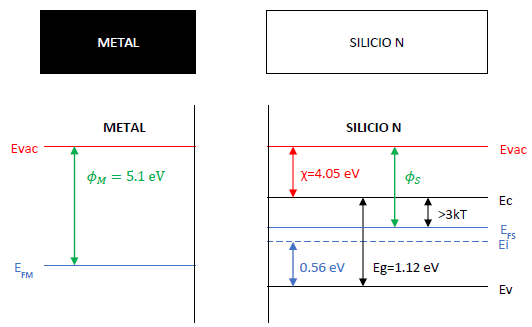
\includegraphics{figuras/contacto_schottky_1.png}
    \caption{Diagramas de bandas de un bloque de metal y un bloque de silicio tipo n por separado.}
    \label{schottky1a}
\end{figure}

Para calcular la función de trabajo del silicio, se observa directamente del diagrama de bandas:

\[ \phi_S = \chi + \dfrac{E_g}{2} - (E_F - E_i) \]

Donde $(E_F - E_i)$ es la posición del nivel de Fermi y depende de la cantidad de dopado.

\textbf{Al unir ambos materiales, el nivel de Fermi del semiconductor se alinea con el del metal.} Debido a que el metal es una superficie equipotencial, las bandas del metal se mantienen fijas, y las bandas del silicio se deben desplazar hacia abajo. Los niveles de energía del semiconductor cambian en la región próxima a la superficie de contacto, para mantener continuidad entre las bandas. Este desplazamiento se muestra en la Figura \ref{schottky1b}:

\begin{figure}[H]
    \centering
    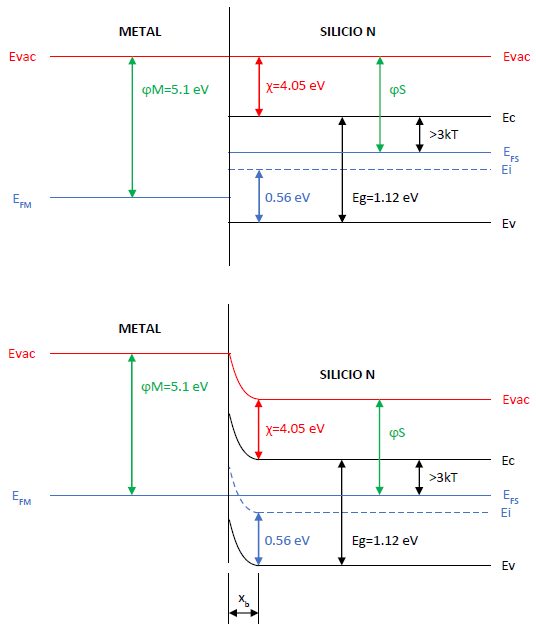
\includegraphics{figuras/contacto_schottky_2.png}
    \caption{Deformación de bandas en el contacto Schottky: se muestran las bandas antes y después del contacto, con la deformación de la región de agotamiento y la carga eléctrica asociada.}
    \label{schottky1b}
\end{figure}

\subsubsection{La barrera Schottky y el potencial de contacto (sin tensión aplicada)}

En la Figura \ref{schottky1c} se muestra la relación que existe entre las variables electrostáticas de este contacto Schottky.

\begin{figure}[H]
    \centering
    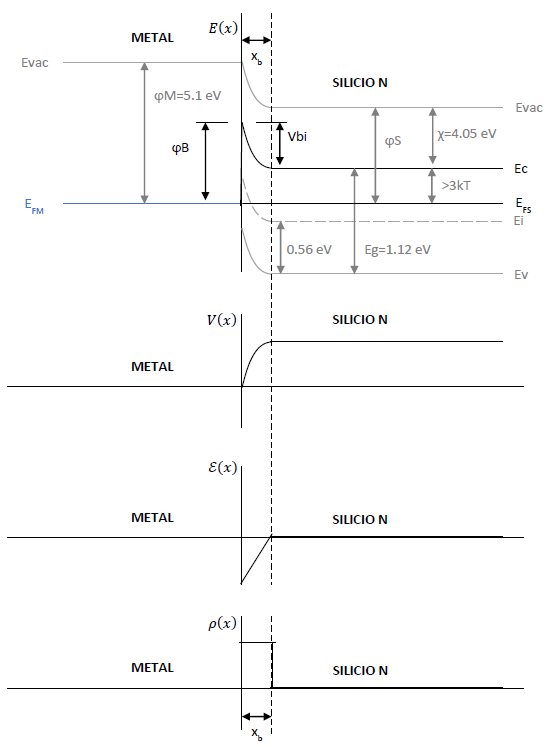
\includegraphics{figuras/contacto_schottky_3.png}
    \caption{Electrostática en un contacto Schottky.}
    \label{schottky1c}
\end{figure}

Analizando la forma que tiene la banda de conducción después de formar el contacto, se aprecia que existe una \textbf{barrera Schottky} ($\phi_B$), que es una barrera de potencial para los electrones que intentan pasar desde el metal hacia el semiconductor. Esta barrera de potencial es imposible de superar, y bloquea el paso de electrones en sentido M-S.

Un contacto Schottky es definido como rectificador debido a que permite el paso de portadores en un solo sentido. En el diagrama se observa que existe un \textbf{potencial de contacto} $V_{bi}$ (también conocido como \textit{Built-in voltage}). Esta tensión es más pequeña que la barrera Schottky, y se puede superar aplicando una tensión externa, logrando conducción de electrones en sentido S-M.

Como se puede observar en la Figura \ref{schottky1d}, existen dos barreras de potencial. 

\begin{itemize}
    \item Para que los electrones puedan pasar del metal al semiconductor, deben superar la barrera Schottky ($\phi_B$). Esta barrera es imposible de superar, por lo que la conducción no es posible en esta dirección.
    \item Para que los electrones puedan pasar del semiconductor al metal, deben superar el potencial de contacto ($V_{bi}$). Esta barrera se puede superar aplicando una tensión externa $V_A$ igual o mayor que el potencial de contacto. La conducción es posible en esta dirección.
\end{itemize}

\begin{figure}[H]
    \centering
    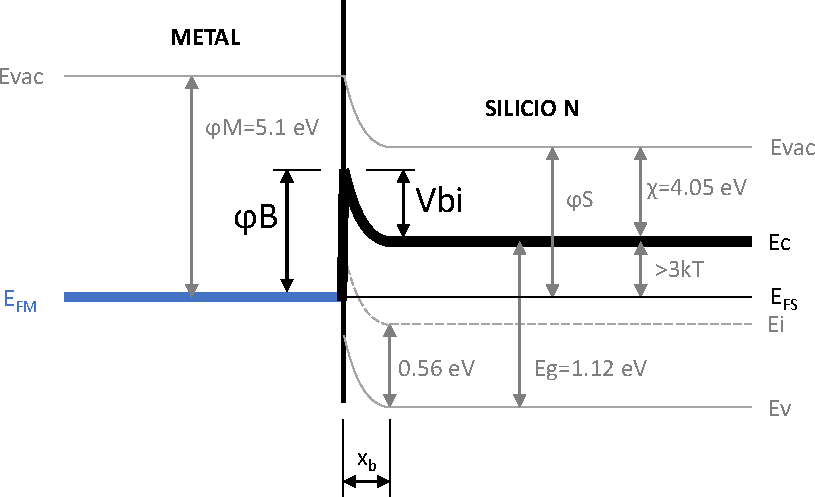
\includegraphics{figuras/contacto_schottky_4.pdf}
    \caption{Diagrama de bandas de un contacto Schottky metal-semiconductor n, después del doblamiento de bandas, haciendo énfasis en la barrera Schottky $\phi_B$ y el potencial de contacto $V_{bi}$.}
    \label{schottky1d}
\end{figure}

La barrera Schottky se calcula como:

\[ \phi_B = \phi_M - \chi \]

El potencial de contacto se calcula como:

\[ V_{bi} = \dfrac{-1}{q} (\phi_M - \phi_S) \]


\newpage
\subsubsection{La barrera Schottky y el potencial de contacto (con tensión aplicada)}

El símbolo del circuito del diodo Schottky es una flecha con una ``S'' cuadrada, como se muestra en la Figura \ref{schottky1e}. El diodo permite la conducción de la corriente convencional en la dirección de la flecha. La terminal positiva se llama \textbf{ánodo}, y se define como la terminal por la que la corriente convencional ingresa a un dispositivo electrónico. La terminal negativa se llama \textbf{cátodo}, definida como la terminal por la cual la corriente convencional sale de un dispositivo electrónico.

Cuando se aplica tensión en sentido positivo, se dice que el diodo opera en \textbf{polarización directa} y existe flujo de corriente. En polarización directa, los electrones del semiconductor NO pueden pasar al metal, a menos que se aplique tensión suficiente para superar una barrera de potencial $V_{bi}$.

 Si se aplica tensión en sentido negativo, el diodo opera en \textbf{polarización reversa}, se bloquea el flujo y la corriente es cero. En polarización reversa, los electrones del metal NO pueden pasar al semiconductor porque existe una barrera $\phi_B$ que no se puede superar.
 

\begin{figure}[H]
    \centering
    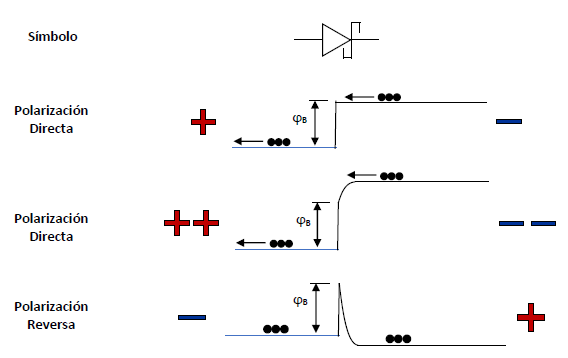
\includegraphics{figuras/contacto_schottky_5.png}
    \caption{Deformación de bandas en un diodo Schottky en polarización directa y reversa.}
    \label{schottky1e}
\end{figure}


\newpage
\subsubsection{Ancho de la región de agotamiento}

La ecuación de Poisson:

\[ \dfrac{d\vec{\mathcal{E}}}{dx} = \dfrac{\rho}{\epsilon_0 \epsilon_r} = \dfrac{q N_D}{\epsilon_0 \epsilon_r} \]

Separando las variables e integrando a ambos lados:

\[ \int_{\mathcal{E}}^{0} d\vec{\mathcal{E}} = \int_x^w \dfrac{q N_D}{\epsilon_0 \epsilon_r} dx \]

\[ \mathcal{E}(x) = \dfrac{-q N_D}{\epsilon_0 \epsilon_r} (w - x) \]

Donde $x$ es una posición arbitraria en el material, y $w$ es el ancho de la región donde se presenta una curvatura o deformación de bandas.

El potencial se obtiene al integrar el campo eléctrico:

\[ \dfrac{dV}{dx} = -\mathcal{E} \]

Separando nuevamente las variables y sustituyendo el resultado anterior:

\[ \int_{V(x)}^{V(w)}  dV = \int_x^w \dfrac{-q N_D}{\epsilon_0 \epsilon_r} (w - x) dx \]

\[ V(w) - V(x) =\dfrac{-q N_D}{\epsilon_0 \epsilon_r} (w - x)^2 dx \]

Sustituyendo $V(w) = V_{bi}$ y $V(x) = V_A$:

\[ w = \sqrt{\dfrac{2 \epsilon_0 \epsilon_r (V_{bi} - V_A)}{q N_D}} \]


\subsubsection{Capacitancia de directa}

Los diodos en reversa son un circuito abierto, y en directa son un corto circuito. Sin embargo, el modelo no ideal del diodo involucra resistencia y capacitancia.

Cuando se polariza en directa, el diodo Schottky tiene una zona de agotamiento con ancho $x_d$.

\begin{itemize}
    \item La densidad de carga existente en la zona de agotamiento es $\rho$.
    \item La permitividad relativa del silicio es $\epsilon_r = 11.9$.
    \item La distancia entre las ``placas'' paralelas de un condensador es $x_d$.
\end{itemize}

Por lo tanto, la capacitancia de directa del diodo Schottky (por unidad de área) es:

\[ C_j = \dfrac{\epsilon_0 \epsilon_r}{x_d} = \sqrt{\dfrac{q \epsilon_0 \epsilon_r N_D}{2 (V_{bi} - V_A)}} \]


\newpage

%\begin{ejemplo}
%Se deposita cobre sobre un sustrato cuidadosamente preparado de silicio n, para formar un diodo Schottky ideal. $\phi_M=4.65\ eV$, $\chi=4.03\ eV$, $N_D=10^{16}\ cm^{-3}$ y $T=300\ K$. Determine:

%\begin{enumerate}
%    \item La barrera Schottky $\phi_B$.
%    \item El potencial de contacto $V_{bi}$.
%    \item El ancho de la región de doblamiento de bandas $w$ si $V_A=0\ V$.
%\end{enumerate}

%Referencia: Pierret, p487.
%\end{ejemplo}

%\begin{solucion}

%1. La barrera Schottky $\phi_B$:

%\[ \phi_B = \phi_M - \chi \]

%\[ \phi_B = 4.65\ eV - 4.03\ eV \]

%\[ \phi_B = 0.62\ eV \]

%2. El potencial de contacto $V_{bi}$:

%\[ V_{bi} = \dfrac{-1}{q}(\phi_M - \phi_S) \]

%Aquí es necesario calcular primero la función de trabajo del silicio:

%\[ \phi_S = \chi + \dfrac{E_g}{2} - (E_F - E_i) \]

%\[ \phi_S = \chi + \dfrac{E_g}{2} - kT \ln \dfrac{N_D}{n_i} \]

%\[ \phi_S = 4.03\ eV + 0.56\ eV - 26\ meV \ln \dfrac{10^{16}}{10^{10}} \]

%\[ \phi_S = 4.23\ eV \]

%De manera que el potencial de contacto es:

%\[ V_{bi} = \dfrac{-1}{q}(4.65\ eV - 4.23\ eV) \]

%\[ V_{bi} = \dfrac{-1}{q}(0.42\ eV) \]

%\[ V_{bi} = 0.42\ V \]

%3. El ancho de la región $w$:

%\[ w = \sqrt{\dfrac{2 \epsilon_0 \epsilon_r (V_{bi} - V_A)}{q N_D}} \]

%\[ w = \sqrt{\dfrac{2 (8.85\times{}10^{-14}\ F/cm) (11.9) (0.42\ V - 0)}{(1.602\times{}10^{-19}\ C) (10^{16}\ cm^{-3})}} \]

%\[ w = 2.35\times{}10^{-5}\ cm \times \dfrac{10^4\ \mu m}{1\ cm} \]

%\[ w = 0.235\ \mu m \]
%\end{solucion}


%\begin{ejemplo}
%Se tiene una unión de cromo-silicio con $N_D=10^{17}\ cm^{-3}$. Si se aplica $V_A=-5\ V$ en la terminal del metal, y la terminal del semiconductor está conectada a tierra, calcule:

%\begin{itemize}
%    \item El potencial de contacto $V_{bi}$.
%    \item El ancho de la región de doblamiento de bandas $w$ sin tensión aplicada.
%    \item La magnitud del campo eléctrico $\mathcal{E}$ en la interfaz ($x=0$).
%    \item El potencial total existente en el diodo $V$.
%    \item La capacitancia de directa por unidad de área $C_j$.
%\end{itemize}

%Referencia: Bart Van Zeghbroek, Principles of Semiconductor Devices, University of Colorado Boulder.
%\end{ejemplo}


\newpage
\subsection{Contacto Schottky metal-silicio n}

El diagrama completo de un contacto Schottky metal-silicio n se muestra en la Figura \ref{contacto_resumen_1}.

\begin{figure}[H]
    \centering
    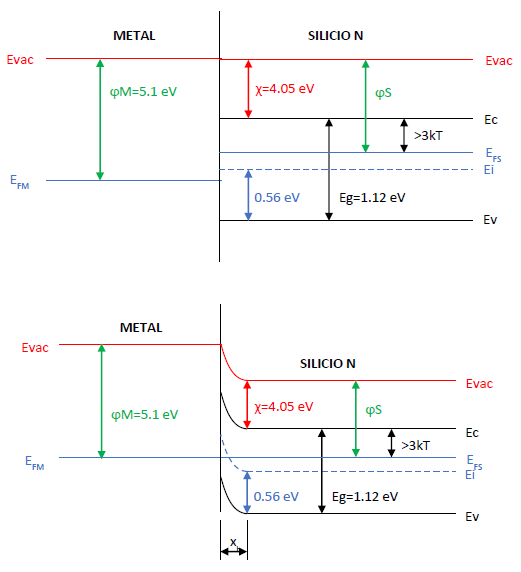
\includegraphics{figuras/contacto_resumen_1.png}
    \caption{Diagrama de bandas de un contacto Schottky metal-silicio n.}
    \label{contacto_resumen_1}
\end{figure}

\newpage
\subsection{Contacto Schottky metal-silicio p}

El diagrama completo de un contacto Schottky metal-silicio p se muestra en la Figura \ref{contacto_resumen_2}.

\begin{figure}[H]
    \centering
    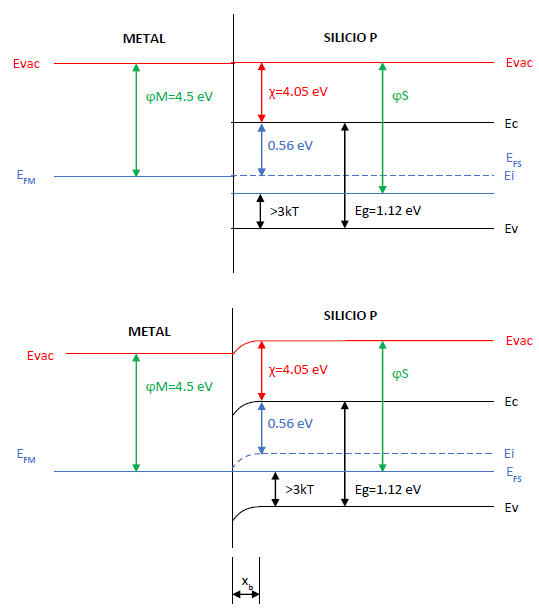
\includegraphics{figuras/contacto_resumen_2.png}
    \caption{Diagrama de bandas de un contacto Schottky metal-silicio p.}
    \label{contacto_resumen_2}
\end{figure}

\newpage
\subsection{Contacto óhmico metal-silicio n}

El contacto óhmico es un contacto de resistencia muy baja, que permite el paso de portadores en ambos sentidos. En uno de los dos sentidos de dirección se tiene una barrera Schottky $\phi_B$ muy baja, para la cual la energía térmica a temperatura ambiente es suficiente para vencer esta barrera. En el otro sentido no se requiere de ningún tipo de energía extra para el traslado de portadores. Una de las aplicaciones más comunes de este tipo de contacto es cuando se utilizan para conectar terminales de transistores en circuitos integrados.

El diagrama completo de un contacto óhmico metal-silicio n se muestra en la Figura \ref{contacto_resumen_3}.

\begin{figure}[H]
    \centering
    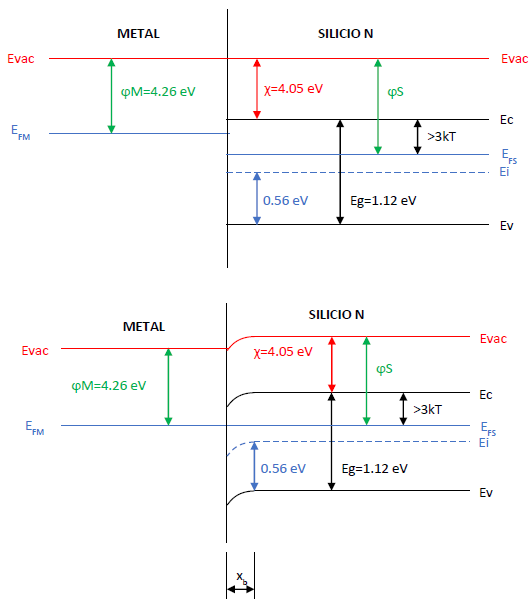
\includegraphics{figuras/contacto_resumen_3.png}
    \caption{Diagrama de bandas de un contacto óhmico metal-silicio n.}
    \label{contacto_resumen_3}
\end{figure}

\newpage
\subsection{Contacto óhmico metal-silicio p}

El diagrama completo de un contacto óhmico metal-silicio p se muestra en la Figura \ref{contacto_resumen_4}.

\begin{figure}[H]
    \centering
    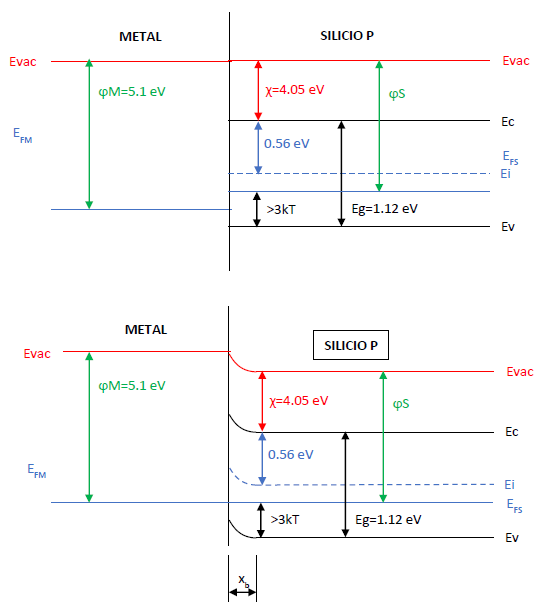
\includegraphics{figuras/contacto_resumen_4.png}
    \caption{Diagrama de bandas de un contacto óhmico metal-silicio p.}
    \label{contacto_resumen_4}
\end{figure}











%\subsection{Curva característica de la unión PN}

%(La curva se puede dejar para el capítulo del diodo)

%\newpage
%\section*{Problemas}

%\textbf{Problema 4.1.} Esboce el diagrama de bandas para un metal con una función de trabajo $\varphi_{M}$ que sea mayor que la de un Semiconductor tipo P. Repita para el caso en que la función de trabajo de un semiconductor $\varphi_{S}$ tipo P, es mayor que la de un metal dado, determine:

%\begin{itemize}
%    \item Los tipos de contacto obtenidos.
%    \item Los diagramas completos antes de la unión y posterior a la unión.
%    \item Complete la tabla con las respectivas relaciones de función de trabajo.
%\end{itemize}

%\begin{table}[h]
%\centering
%\begin{tabular}{|c|c|l|}
%\hline
%\textbf{Contacto} & \textbf{Óhmico} & \multicolumn{1}{c|}{\textbf{Schottky}}             \\ \hline
%Tipo N &  & $\varphi_{M}$ > $\varphi_{S}$                                   
%\\ \hline
%Tipo P &  &
%\\ \hline
%\end{tabular}
%\end{table}


